\documentclass[11pt]{article}

\usepackage[margin=1in]{geometry}
\usepackage{booktabs}
\usepackage{amsmath,amssymb}
\usepackage{microtype}
\usepackage{natbib}
\usepackage{graphicx}
\usepackage{xcolor}
\usepackage{pgfplots}
\pgfplotsset{compat=1.18}
\usepackage{float}
\usepackage[colorlinks=true,linkcolor=black,citecolor=black,urlcolor=blue]{hyperref}

\newcommand{\stddeck}{\textsc{Standard}}
\newcommand{\intdeck}{\textsc{Interactive}}
\newcommand{\searchn}[1]{\textsc{search}-#1}
\newcommand{\ci}[2]{\,[#1,\,#2]}
\newcommand{\draftnote}[1]{\textcolor{gray}{\small\itshape[#1]}}

\title{\textbf{manabot}: A Cost-Indexed Study of Search and Learning\\ in a Reduced \textit{Magic: The Gathering}}

\author{Jack Heart\\ \small Loopflow Studio}

\date{\today\\[0.5em]\small\textit{Working draft --- a standing snapshot of what the project can currently defend.}}

\begin{document}
\maketitle

\begin{abstract}
We describe \textbf{manabot}, a research system for reinforcement learning on a reduced subset of \textit{Magic: The Gathering}, and report what it has actually established. The system pairs \textbf{managym}, a deterministic, seedable, forkable Rust game engine ($\approx$10.7k lines, 35 cards, 106 rules-cited tests) exposing a Gymnasium-compatible vectorized API at $1.8\times10^{5}$ environment steps/second, with a PPO learner and a flat determinized Monte Carlo (PIMC) search player sharing one observation encoding.

The empirical contribution is negative and, we argue, more useful than a win-rate claim. Under seat-balanced evaluation with pre-registered predictions, we find that (i) naive on-the-play seat advantage is so large --- $94.1\%\ci{92.5\%}{95.4\%}$ for random-vs-random on a creature deck --- that unbalanced win rates measure seating, not skill, invalidating our own prior results; (ii) every policy we trained with PPO from scratch sits \emph{below} a 16-simulation-per-action flat search that costs \$0 to train and 7\,ms per decision; (iii) behavior cloning from that search reaches $90.5\%\ci{87.2\%}{93.0\%}$ against random for \$0.66 of compute, beating a cost-matched PPO run at $52.7\%\ci{47.9\%}{57.6\%}$; and (iv) the dense per-event reward shaping our project was founded on is \emph{worse than no shaping at all}, and the pass-collapse pathology it was introduced to fix does not replicate. The right amount of reward shaping here is approximately zero.

We publish the ledger of refuted claims alongside the surviving ones. Several sections of this paper document capability the system does not yet have.
\end{abstract}

\section{Introduction}

\textit{Magic: The Gathering} is an unusually hostile target for reinforcement learning. It is an imperfect-information game with hidden hands and hidden library order; it has a legal action set that varies in size and meaning at every decision point; its card pool is effectively unbounded and its rules are Turing complete \citep{churchill2019turing}. It is also, unlike poker, not a game whose strategic content survives abstraction: the interesting decisions are precisely the ones that depend on which specific cards exist.

Most published game-RL results arrive as a headline win rate against a strong reference \citep{silver2018alphazero,vinyals2019starcraft,bakhtin2022cicero}. This paper is not that. \textbf{manabot} is a small, self-funded system, and at the scale it operates the dominant question is not ``can a network beat a grandmaster'' but ``does any of this work at all, and how would we know.'' Our experience has been that the second question is far harder than it looks, and that the majority of our early results were measurement artifacts.

This paper therefore has two halves. Sections \ref{sec:managym}--\ref{sec:manabot} describe the artifact: a Rust engine designed from the start for cloning, seeding, and determinization, and a Python learner that shares one observation encoder between a PPO policy and a search player. Sections \ref{sec:method}--\ref{sec:refuted} describe the experimental ledger: a sequence of pre-registered cycles, each with a written prediction and a cost cap, most of which refuted something we previously believed --- including, on three occasions, a belief on which the project's direction had been staked.

\paragraph{Contributions.}
\begin{enumerate}\itemsep2pt
\item A deterministic, forkable MTG engine with first-class determinization primitives, making PIMC search a native operation rather than a bolt-on (\S\ref{sec:determinize}).
\item A measurement protocol --- seat-balanced evaluation, Wilson intervals, pre-registered predictions, and a dollar-denominated cost axis --- under which we can state that a result is real (\S\ref{sec:method}).
\item Evidence that at our scale, \textbf{search dominates learning}: no PPO policy we trained beats a 16-sim flat search, and distilling that search is $\approx$6$\times$ cheaper per unit of strength than PPO (\S\ref{sec:search}--\ref{sec:distill}).
\item Evidence that \textbf{potential-based shaping $\approx$ terminal-only $\gg$ per-event shaping}, and that the pass-collapse pathology motivating per-event shaping does not replicate (\S\ref{sec:shaping}).
\item A published table of our own refuted claims (\S\ref{sec:refuted}).
\end{enumerate}

\section{Related Work}

\paragraph{Determinized search in imperfect-information games.} Perfect-Information Monte Carlo (PIMC) --- sample a world consistent with your information set, solve it as if perfect-information, average --- is the classical workhorse for trick-taking card games, most famously in bridge \citep{ginsberg2001gib}. Its known pathologies are \emph{strategy fusion} and \emph{non-locality} \citep{frank1998bridge}; \citet{long2010pimc} characterize the game properties under which PIMC nonetheless performs well. Information Set MCTS \citep{cowling2012ismcts} addresses fusion by searching over information sets directly. \citet{cowling2012magic} apply ensemble determinization to \textit{Magic} specifically, and remain the closest prior work to our search player. We use flat (depth-1) determinized MC with uniform rollouts --- strictly weaker than any of these --- as a deliberately cheap baseline, and it is already stronger than everything we trained.

\paragraph{Search distillation and expert iteration.} Distilling a search procedure into a fast reactive policy is an old and reliable idea \citep{guo2014uctdistill}, generalized by expert iteration \citep{anthony2017exit} and AlphaZero \citep{silver2018alphazero}, and extended to imperfect information by ReBeL \citep{brown2020rebel}. Our \S\ref{sec:distill} is a single iteration of the simplest version of this (one round of behavior cloning, no DAgger \citep{ross2011dagger}, no value target), reported mainly because of how favorably it compares to the RL baseline.

\paragraph{Reward shaping.} \citet{ng1999shaping} give the potential-based form $\gamma\Phi(s')-\Phi(s)$ that provably preserves the optimal policy. Our \S\ref{sec:shaping} is a direct empirical test of policy-invariant against non-invariant shaping in a setting where the non-invariant version was believed to be necessary.

\paragraph{Reproducibility in deep RL.} \citet{henderson2018matters} document how sensitive deep-RL conclusions are to seeds, implementation, and evaluation protocol. Our seat-contamination finding (\S\ref{sec:seat}) is a domain-specific instance of exactly their warning, and we found it only after building the protocol to look.

\section{managym: The Environment}
\label{sec:managym}

\subsection{Scope}

\textbf{managym} implements a two-player subset of the \textit{Comprehensive Rules} in Rust ($\approx$10{,}738 lines under \texttt{src/}), with PyO3 bindings. Table~\ref{tab:rules} summarizes coverage as tracked in \texttt{docs/rules\_coverage.yaml}. The subset is chosen to be closed: everything in it is tested, and nothing in the card pool depends on anything outside it.

\begin{table}[t]
\centering\small
\begin{tabular}{llp{6.6cm}}
\toprule
\textbf{CR section} & \textbf{Status} & \textbf{Notes / known gap} \\
\midrule
103 Game start & tested & Opening hand of seven; \textbf{no mulligans} \\
106 Mana & tested & Deterministic auto-tap; no floating-mana choice \\
117 Priority & tested & APNAP pass loop; all-pass advances step \\
305 Lands & tested & One per turn; no additional-land effects \\
601 Casting (subset) & tested & Timing/cost legality for the current pool \\
508/509 Attack, block & tested & Per-creature declaration; \textbf{single-block only} \\
510 Combat damage & tested & First/double strike, trample, deathtouch, menace \\
514 Cleanup, 704.5 SBAs & tested & Life $\le 0$, empty draw, lethal damage, token cleanup \\
603 Triggers & tested & Data-driven; see \S\ref{sec:triggers} \\
\midrule
Layers, replacement/prevention & \textbf{absent} & Designed, not implemented \\
Multiplayer, planeswalkers, battles & \textbf{absent} & \texttt{Game::new} asserts exactly two players \\
\bottomrule
\end{tabular}
\caption{Rules coverage. ``tested'' means a CR-cited integration test exists under \texttt{managym/tests/rules/} (106 such tests). The absences are load-bearing: they bound every claim in this paper.}
\label{tab:rules}
\end{table}

The card pool is 35 registered cards: five basic lands, 18 from Alpha (including \textit{Lightning Bolt}, \textit{Counterspell}, \textit{Ancestral Recall}, \textit{Shivan Dragon}), \textit{Pyroclasm}, \textit{Man-o'-War}, and a ten-card slice exercising modern mechanics (tokens, $+1/+1$ counters, flash, ETB triggers with subject predicates). Two decklists are used throughout:

\begin{itemize}\itemsep1pt
\item \stddeck: 12 Mountain, 12 Forest, 18 Llanowar Elves, 18 Grey Ogre. Zero interaction --- a pure race.
\item \intdeck: 12 Island, 12 Mountain, 20 creatures, and 16 interaction spells (6 Lightning Bolt, 4 Counterspell, 3 Ancestral Recall, 3 Pyroclasm). Instants make timing matter.
\end{itemize}

The choice of two decks is itself a result: \S\ref{sec:shaping} shows that a policy trained with terminal reward alone adapts its behavior to the deck, and that the shaping we had been using forced \stddeck{} behavior onto \intdeck.

\subsection{State, actions, observations}

The engine's central loop (\texttt{flow/tick.rs}) advances turn structure, grants priority under APNAP, and surfaces a decision only when one exists. An \texttt{ActionSpace} is a \emph{variable-length list of legal actions} together with a \texttt{kind} (\texttt{Priority}, \texttt{DeclareAttacker}, \texttt{DeclareBlocker}, \texttt{ChooseTarget}); the agent selects by integer index into that list. There is no fixed global action vocabulary --- index $i$ means nothing across states. Each action additionally carries a \texttt{focus} set: the object IDs it refers to (the card cast, the creature blocked, the target chosen), which the policy consumes directly (\S\ref{sec:net}).

A flag \texttt{skip\_trivial} collapses any decision point with $\le 1$ legal action. Across $\approx$311k recorded decisions we observed \emph{zero} decisions surviving with $\le 1$ valid action, confirming the collapse is exact. It is also less consequential than we assumed: it removes only $12.4\%$ of decision points (\S\ref{sec:profile}).

Observations are hidden-information correct: the opponent's hand and both libraries are never listed. The encoder (\texttt{agent/observation\_encoder.rs}) emits a fixed-width padded tensor set with parallel validity masks --- per-player $[27]$, per-card $[60\times33]$, per-permanent $[30\times7]$, actions $[20\times8]$, events $[32\times7]$, and \texttt{action\_focus} $[20\times2]$ of \texttt{i32} indices into a per-observation object table. Card features carry zone one-hot, ownership, P/T/mana value, six type flags, twelve keyword flags, and token/tribal tags.

\subsection{Determinization and search primitives}
\label{sec:determinize}

This is the design decision the rest of the paper rests on. All randomness flows through a single \texttt{ChaCha8Rng} in \texttt{GameState}, so a \texttt{(decklists, seed)} pair fully determines a game; \texttt{Game::reseed} can redirect the stream at any point; and \texttt{Env::fork()} produces a fully independent deep clone (verified by test).

Because decklists are mutually known in constructed \textit{Magic}, the hidden state is exactly the opponent's hand plus both library orders. \texttt{Game::determinize(perspective, seed)} therefore samples from the belief state directly: it pools the opponent's hand with their library, shuffles, re-deals to preserve the observed hand size, reshuffles the perspective player's library, and preserves every public zone and the current \texttt{ActionSpace}.

On top of this the engine exposes \texttt{flat\_mc\_scores(worlds, rollouts, seed, max\_steps)}: for each legal action, sample $W$ determinized worlds, apply the action to a clone, and score by $R$ uniform-random playouts to a true terminal (win $1$, loss $0$, draw-or-cap $\tfrac12$). Worlds are shared across actions as common random numbers to reduce comparison variance. \emph{Search is an engine primitive, not a Python loop} --- this is why \S\ref{sec:search} costs 4.5 CPU-core-hours instead of a week.

\subsection{Throughput}

Measured on an Apple M4 Max. Environment stepping alone: $90{,}898$ steps/s at one environment, $183{,}350\pm660$ at sixteen, saturating near $1.9\times10^{5}$. With policy inference in the loop this falls to $2{,}035$ steps/s --- inference is $\approx$72$\times$ the cost of the environment --- and with the full PPO update, to $2{,}472$--$2{,}856$ steps/s. \textbf{The environment is not the bottleneck and has not been since early 2026.} We note this because it inverts the usual assumption for board-game RL and because it is what makes the cost accounting in \S\ref{sec:cost} dominated by learning, not simulation.

Attempts to parallelize the vector environment with Rayon were performance-neutral to negative; the shipping implementation is single-threaded per environment.

\subsection{The trigger substrate}
\label{sec:triggers}

Triggered abilities are fully data-driven: an \texttt{Ability::Triggered\{condition, effects\}} where \texttt{TriggerCondition} ranges over ETB / dies / attacks / becomes-tapped / tapped-for-mana / upkeep / ``you draw your $n$th card this turn'', each parameterized by a \texttt{TriggerSubject} (\texttt{This}, \texttt{AnotherYouControl(pred)}, \texttt{AnyYouControl(pred)}) over a structural \texttt{CardPredicate}. Effects compose, including a recursive \texttt{OnNthResolutionThisTurn} gate. Triggers are collected from game events, ordered APNAP, dropped if no legal target exists (CR 603.3d), and placed on the stack. This is the substrate that must generalize if the card pool is ever to grow past 35; whether it does is untested.

\section{manabot: The Learning System}
\label{sec:manabot}

\subsection{Policy--value network}
\label{sec:net}

One \texttt{Agent} class, 100{,}354 parameters (50{,}306 with attention disabled). Typed projections embed each object class into $d=64$: players $27\to64$, cards $33\to64$, permanents $7\to64$, actions $7\to64$. When attention is enabled, all objects are concatenated into a single sequence, a learned \emph{perspective} vector is added with its sign flipped by ownership ($+1$ mine, $-1$ theirs), and one post-LN transformer block \citep{vaswani2017attention} with four heads and a key-padding mask from the validity vectors mixes them.

Variable-length action scoring is deliberately \emph{not} a pointer network \citep{vinyals2015pointer}. Each action embedding is concatenated with the post-attention embeddings of its $\le2$ focus objects ($3\times64=192$ dims), projected to $64$, and scored by a shared two-layer head to one logit per action slot; invalid slots are masked to $-10^8$ and the policy is a categorical over the $\le20$ slots. The value head mean-pools objects. This buys permutation-equivariance over the action list and lets the policy condition on \emph{what an action does to which object} without a decoder.

\subsection{PPO}

A CleanRL-style flat PPO \citep{huang2022cleanrl,schulman2017ppo} over the vectorized environment, with GAE \citep{schulman2015gae}. Defaults: $\gamma=0.99$, $\lambda=0.95$, lr $2.5\times10^{-4}$ (linearly annealed), 16 environments $\times$ 128 steps, 4 minibatches, 4 epochs, clip $0.1$, entropy coefficient $0.01$, value coefficient $0.5$, gradient clip $0.5$.

One number matters for interpreting everything downstream: the GAE effective horizon is $1/(1-\gamma\lambda)\approx16.8$ steps, while a policy surfaces 91--106 decisions per game against an active opponent (\S\ref{sec:profile}). \textbf{Credit must travel roughly six horizons to reach the terminal reward.} This was the original motivation for dense shaping, and \S\ref{sec:shaping} shows the inference was wrong.

\subsection{Reward regimes}

Three, selected by config, all sharing $+1$ win / $-1$ loss:
\begin{itemize}\itemsep1pt
\item \textbf{Terminal-only.} Nothing else.
\item \textbf{Per-event (``pay-per-event'').} $+0.03$ per land played, $+0.06$ per creature resolved, $+0.01$ per point of opponent life lost. Path-dependent, not policy-invariant. This was the project's founding recipe, \texttt{first\_light\_shaped\_v1}.
\item \textbf{Potential-based} \citep{ng1999shaping}. $\gamma\Phi(s')-\Phi(s)$ with $\Phi(s)=0.03\Delta_{\text{lands}}+0.06\Delta_{\text{creatures}}+0.2(\ell_{\text{hero}}-\ell_{\text{villain}})/20$ and $\Phi(\text{terminal})=0$. Weights matched to the per-event magnitudes so that \emph{form}, not scale, is the manipulated variable.
\end{itemize}

\subsection{Search player and distillation}

\texttt{FlatMCPlayer} wraps the engine primitive: strength dial $N$ = simulations per legal action, split as $W=\lfloor N/R\rfloor$ worlds $\times$ $R{=}4$ rollouts, playout cap 2000 steps, then $\arg\max$. No tree, no network, no value function --- this is the weakest search worth the name.

Distillation (\texttt{manabot/sim/distill.py}) is pure behavior cloning: play \searchn{64} against itself, record every decision by both seats as (encoded observation, teacher's $\arg\max$ index), and minimize cross-entropy through the student's own masked logits. Train/validation split is \emph{by game} to prevent within-game leakage. No soft targets, no value loss, no DAgger.

\section{Methodology: Making Any Claim At All}
\label{sec:method}

\subsection{The cycle}

Work proceeds in numbered cycles. Each begins with a written question, a \emph{pre-registered prediction}, and a cost cap; each ends with a report in \texttt{experiments/} recording whether the prediction held. Of the seven predictions registered so far, three were refuted, one was confirmed but in the wrong direction, and three held. We report all of them.

\subsection{Seat contamination}
\label{sec:seat}

The engine hard-codes \texttt{PlayerId(0)} on the play (implementing CR 103.7.1's first-turn draw skip). Our early evaluations put the hero in seat 0 always. The consequence, measured on 1000 seat-balanced random-vs-random games:

\begin{center}\small
\begin{tabular}{lccc}
\toprule
Deck & On the play & On the draw & Overall (balanced) \\
\midrule
\stddeck  & $94.1\%\ci{92.5}{95.4}$ & $5.9\%$ & $50.3\%\ci{47.2}{53.4}$ \\
\intdeck  & $23.1\%\ci{20.6}{25.8}$ & $76.9\%$ & $48.9\%\ci{45.8}{52.0}$ \\
\bottomrule
\end{tabular}
\end{center}

On the creature deck, going first wins $94\%$ of games \emph{between two uniformly random players}. On the interactive deck the advantage \textbf{inverts}: going first \emph{loses} $77\%$ of the time, because a random agent on the play walks its creatures into an untapped opponent. Either way, a hero-on-play win rate is a measurement of the seat.

This retroactively destroyed our founding result. The original ``$82\%$ against random'' was a seat reading. Worse, an apparent ``13\%--89\% spread across three network initializations'' --- which we had written up as evidence of catastrophic init sensitivity --- vanished under balancing: across eight inits and both decks, seat-balanced win rates for \emph{untrained} networks span $48.2\%$--$51.7\%$ and every Wilson interval covers $50\%$. The spread was a seat-by-init interaction. Per-seat rates for a single untrained network ranged from $1.5\%$ to $100\%$.

Everything reported below is seat-balanced: the hero plays seat 0 on even game indices and seat 1 on odd, and we report overall and per-seat rates with Wilson intervals \citep{wilson1927}.

\subsection{The gate}

From this we fixed a success criterion in advance, replacing the withdrawn ones: a policy \emph{passes} if, over $\ge400$ seat-balanced games against a uniformly random opponent on \intdeck, its Wilson $95\%$ lower bound exceeds $55\%$ overall \emph{and} its win rate exceeds $50\%$ in each seat separately. The second clause exists to kill seat-parasitic policies, which we then promptly produced (\S\ref{sec:c1}).

\subsection{Ladder strength and the cost axis}
\label{sec:cost}

We index strength not by win rate against random --- which saturates --- but by \textbf{ladder strength}: the largest $N$ such that the policy, alone and without search, beats \searchn{N} head-to-head. \searchn{N} is a well-defined, training-free, monotone ladder (we verify monotonicity in \S\ref{sec:search}), and $N$ is directly interpretable as ``how much thinking this policy is worth.''

The cost axis is dollars. We book compute at the AWS \texttt{g5.xlarge} on-demand rate (\$1.006/hr, \texttt{us-west-2}). At the measured $637$ training steps/s of the era, $10^6$ steps $=$ \$0.44. Actual marginal cost on the laptop these ran on is electricity, roughly \$0.10--0.15 for the entire experimental program; the booked number is a fiction we maintain so that the strength-per-dollar comparisons are portable. We flag it as a fiction rather than launder it.

\begin{figure}[t]
\centering
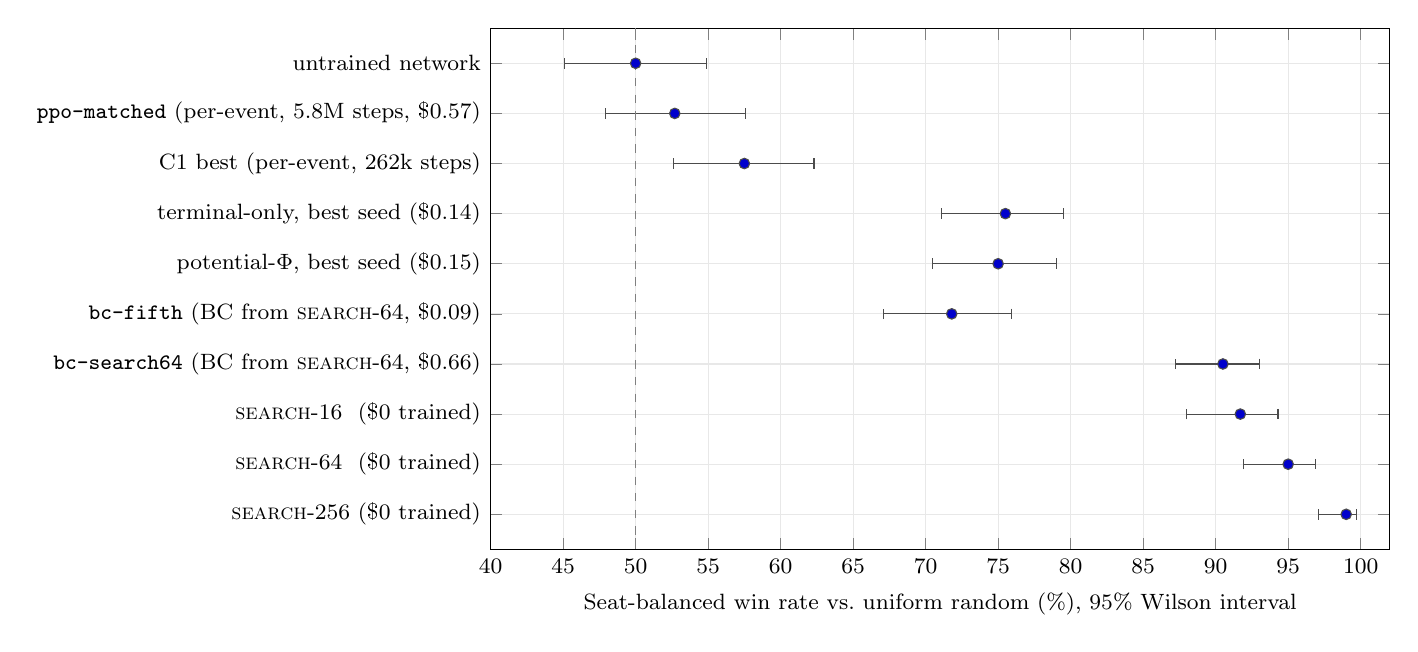
\begin{tikzpicture}
\begin{axis}[
  width=13cm, height=8.2cm,
  xlabel={Seat-balanced win rate vs.\ uniform random (\%), 95\% Wilson interval},
  xmin=40, xmax=102,
  ytick={0,...,9},
  yticklabels={
    {untrained network},
    {\texttt{ppo-matched} (per-event, 5.8M steps, \$0.57)},
    {C1 best (per-event, 262k steps)},
    {terminal-only, best seed (\$0.14)},
    {potential-$\Phi$, best seed (\$0.15)},
    {\texttt{bc-fifth} (BC from \searchn{64}, \$0.09)},
    {\texttt{bc-search64} (BC from \searchn{64}, \$0.66)},
    {\searchn{16} \ (\$0 trained)},
    {\searchn{64} \ (\$0 trained)},
    {\searchn{256} (\$0 trained)}},
  y dir=reverse, ymin=-0.7, ymax=9.7,
  grid=major, grid style={gray!18},
  tick label style={font=\footnotesize},
  label style={font=\footnotesize},
  yticklabel style={align=right},
]
\addplot+[only marks, mark=*, mark size=1.9pt, color=black!70,
  error bars/.cd, x dir=both, x explicit]
table[x=v, y=i, x error minus=em, x error plus=ep, row sep=\\] {
v i em ep \\
50.0 0 4.9 4.9 \\
52.7 1 4.8 4.9 \\
57.5 2 4.9 4.8 \\
75.5 3 4.4 4.0 \\
75.0 4 4.5 4.0 \\
71.8 5 4.7 4.1 \\
90.5 6 3.3 2.5 \\
91.7 7 3.7 2.6 \\
95.0 8 3.1 1.9 \\
99.0 9 1.9 0.7 \\
};
\draw[dashed, gray] (axis cs:50,-0.7) -- (axis cs:50,9.7);
\end{axis}
\end{tikzpicture}
\caption{Everything we have built, on one axis. Training dollars buy remarkably little; a \$0 search buys a great deal. The three cheapest \emph{trained} policies that are any good (terminal-only, potential-$\Phi$, \texttt{bc-fifth}) all cost under \$0.16. The founding recipe (per-event shaping) is the worst trained configuration on the chart.}
\label{fig:winrate}
\end{figure}

\section{Results}

\subsection{The decision profile}
\label{sec:profile}

Pre-registered prediction: surfaced decisions per game between 40 and 120; hero share below 60. \textbf{Both clauses refuted.} On \stddeck, random-vs-random surfaces $194.1\ci{191.2}{197.1}$ decisions per game across both seats ($106.0$ for the hero), over $40.8$ turns. Combat declarations are $58\%$ of them; \texttt{skip\_trivial} collapses only $12.4\%\ci{12.1}{12.6}$ of decision points, not the large majority we had assumed.

Switching to \intdeck{} changes the shape, not merely the size: hero decisions fall to $0.60\times$, attacker declarations to $0.25\times$ and blocker declarations to $0.10\times$, while priority decisions hold constant and the priority \emph{share} rises from $41.9\%$ to $71.0\%$. Targeting decisions appear for the first time. Our prediction that total decisions would \emph{rise} on the interactive deck was refuted; they fall, because games end faster and creatures rarely survive to attack.

\subsection{PPO from scratch fails the gate}
\label{sec:c1}

We ran the founding recipe unchanged on \intdeck: three seeds, 262k steps each, random opponent, per-event shaping. Judged at 400 seat-balanced games:

\begin{center}\small
\begin{tabular}{lcccccc}
\toprule
Seed & Overall & Wilson LB & On play & On draw & \texttt{cast\_when\_able} & Verdict \\
\midrule
1 & $56.5\%$ & $.516$ & $66.5\%$ & $46.5\%$ & $0.88$ & FAIL \\
2 & $47.3\%$ & $.424$ & $64.5\%$ & $30.0\%$ & $0.95$ & FAIL \\
3 & $57.5\%$ & $.526$ & $20.0\%$ & $95.0\%$ & $0.50$ & FAIL \\
\bottomrule
\end{tabular}
\end{center}

Zero of three pass. Seed 3 is the seat-parasite the gate was designed to catch: its $95\%$ on the draw beats random's $76.9\%$, but its $20\%$ on the play is \emph{worse} than random's $23.1\%$. It learned the seat, not the game.

We also recorded a behavioral fingerprint. \texttt{cast\_when\_able} --- the fraction of priority decisions on which a castable spell is cast --- sits at $0.88$--$0.95$ for these policies. The founding recipe had used $\texttt{cast\_when\_able}\ge0.70$ as a \emph{success criterion}. On the interactive deck, one seed trained from $44\%$ (untrained) down to an $18\%$ win rate while driving \texttt{cast\_when\_able} to $0.96$: the metric flipped sign the moment the game acquired strategy. Holding \textit{Counterspell} is the whole point of \textit{Counterspell}.

\subsection{Search is free, and it wins}
\label{sec:search}

We then measured flat determinized MC against random and against every trained policy: 13 matchups, 3{,}900 seat-balanced games, $77.9$M playouts, $0$ cap-hits, $0$ draws, $4.5$ CPU-core-hours, and \$0 of training.

\begin{center}\small
\begin{tabular}{lcccc}
\toprule
& \multicolumn{1}{c}{vs.\ random} & \multicolumn{3}{c}{vs.\ trained (C1v2 seeds 1/2/3)} \\
\cmidrule(lr){2-2}\cmidrule(lr){3-5}
& Overall & $s_1$ & $s_2$ & $s_3$ \\
\midrule
\searchn{16}\ \ (7\,ms/dec)   & $91.7\%\ci{88.0}{94.3}$ & $92.7\%$ & $89.0\%$ & $84.0\%$ \\
\searchn{64}\ \ (31\,ms/dec)  & $95.0\%\ci{91.9}{96.9}$ & $94.0\%$ & $95.7\%$ & $95.3\%$ \\
\searchn{256} (113\,ms/dec)   & $99.0\%\ci{97.1}{99.7}$ & $98.7\%$ & $98.0\%$ & $97.0\%$ \\
\bottomrule
\end{tabular}
\end{center}

Every trained policy loses to the cheapest search, in every seat (no matchup-seat below $80.7\%$). The ladder is monotone: \searchn{256} beats \searchn{16} $76.7\%\ci{71.6}{81.1}$. Therefore \textbf{every policy we had trained has ladder strength below $N=16$}, and most plausibly $\lesssim1$.

The searcher's fingerprint is the inverse of the trained policies': \texttt{cast\_when\_able} falls from $0.64$ at $N=16$ to $0.52$ at $N=256$. \emph{The better it searches, the less it casts.} The shaped policies had been trained to do the opposite.

This cycle also surfaced an engine bug --- spells with no legal target were stranded in the stack zone forever --- found by random playouts, not by 106 rules tests. Fixed per CR 608.2b.

\begin{figure}[t]
\centering
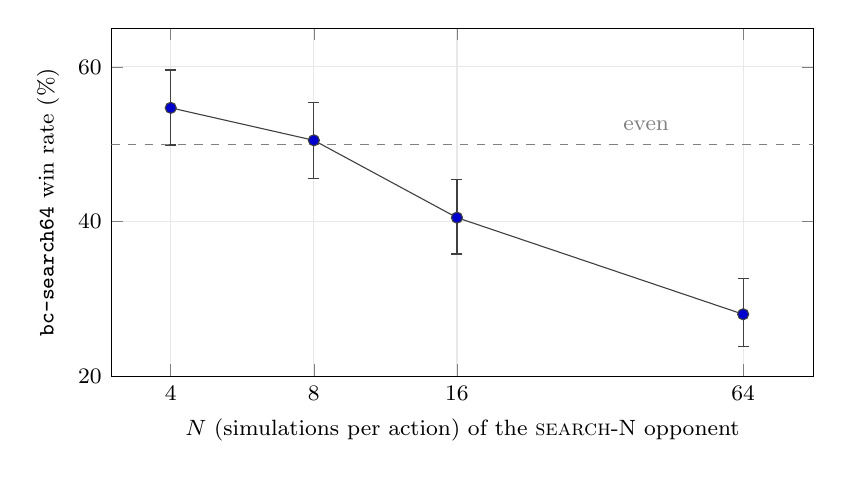
\begin{tikzpicture}
\begin{axis}[
  width=10.5cm, height=6cm,
  xlabel={$N$ (simulations per action) of the \searchn{N} opponent},
  ylabel={\texttt{bc-search64} win rate (\%)},
  xmode=log, log basis x=2, xmin=3, xmax=90,
  ymin=20, ymax=65, xtick={4,8,16,64},
  xticklabels={4,8,16,64},
  grid=major, grid style={gray!18},
  tick label style={font=\footnotesize}, label style={font=\footnotesize},
]
\addplot+[mark=*, mark size=2pt, color=black!75, error bars/.cd, y dir=both, y explicit]
table[x=n, y=w, y error minus=em, y error plus=ep, row sep=\\] {
n w em ep \\
4  54.7 4.8 4.9 \\
8  50.5 4.9 4.9 \\
16 40.5 4.7 4.9 \\
64 28.0 4.2 4.6 \\
};
\draw[dashed, gray] (axis cs:3,50) -- (axis cs:90,50);
\node[font=\footnotesize, gray] at (axis cs:40,52.4) {even};
\end{axis}
\end{tikzpicture}
\caption{Ladder strength of the distilled student: the crossing of the $50\%$ line lies between $N=8$ and $N=16$. Distilling a 31\,ms teacher into a $0.98$\,ms student costs roughly a factor of eight in search-equivalent strength. Every PPO policy we trained lies to the left of $N=4$.}
\label{fig:ladder}
\end{figure}

\subsection{Distilling search beats training from scratch}
\label{sec:distill}

Teacher: \searchn{64}. Dataset: 600 self-play games, $73{,}443$ decisions, mean $3.08$ valid actions per decision. Student: a fresh network, behavior-cloned. Validation accuracy $0.5114$ against $0.389$ for uniform-over-valid. Total cost \$0.66.

Baseline: PPO given \emph{the same wall-clock budget} --- \$0.571, which at the then-current $2{,}856$ steps/s bought $5.84$M timesteps, $22\times$ more experience than any prior run on this deck.

\begin{center}\small
\begin{tabular}{lccc}
\toprule
Matchup (400 seat-balanced games) & Overall & On play & On draw \\
\midrule
\texttt{bc-search64} vs.\ random        & $\mathbf{90.5\%}\ci{87.2}{93.0}$ & $91.5\%$ & $89.5\%$ \\
\texttt{ppo-matched} vs.\ random        & $52.7\%\ci{47.9}{57.6}$ & $41.5\%$ & $64.0\%$ \\
\texttt{bc-search64} vs.\ \texttt{ppo-matched} & $\mathbf{82.0\%}\ci{77.9}{85.5}$ & $66.5\%$ & $97.5\%$ \\
\bottomrule
\end{tabular}
\end{center}

The student's ladder strength is $N\approx8$: it beats \searchn{4} ($54.7\%$) and \searchn{8} ($50.5\%$), loses to \searchn{16} ($40.5\%$) and to its own teacher ($28.0\%$) --- see Figure~\ref{fig:ladder}. It does this at $0.98$\,ms per decision against the teacher's $31$\,ms, a $32\times$ speedup for roughly a threefold loss of ladder position. A one-fifth-scale replication (\texttt{bc-fifth}, \$0.092 --- $1/6.2$ of the PPO budget) still reaches $71.8\%\ci{67.1}{75.9}$.

The student also inherits the teacher's temperament: \texttt{cast\_when\_able} $0.61$ against the teacher's $0.58$, where the cost-matched PPO run sits at $0.97$.

\paragraph{An honest correction.} The \texttt{ppo-matched} baseline used the per-event shaping recipe that \S\ref{sec:shaping} goes on to convict. Against a \emph{well-configured} PPO (terminal-only, $60.0$--$75.5\%$), the honest headline is that behavior cloning beats good PPO by $\approx$15 points at equal cost, not by 38. The direction survives; the margin was inflated by our own bad baseline. We leave both numbers in.

\subsection{The right amount of shaping is approximately zero}
\label{sec:shaping}

The project was founded on a claim, recorded without a supporting experiment: \emph{pure terminal reward fails, producing pass-collapse --- a policy that passes priority forever.} Per-event shaping existed to fix this. We finally tested it.

\begin{center}\small
\begin{tabular}{lccc}
\toprule
Reward (3 seeds) & Mean win rate & Range & \texttt{cast\_when\_able} \\
\midrule
Per-event shaping (the founding recipe) & $52.4\%$ & $43.2$--$58.3$ & $0.88$--$0.95$ \\
Potential-based $\Phi$                   & $\mathbf{69.5\%}$ & $65.2$--$75.0$ & $0.35$--$0.38$ \\
Terminal-only                            & $66.7\%$ & $60.0$--$75.5$ & $0.15$--$0.29$ \\
\bottomrule
\end{tabular}\\[2pt]
{\footnotesize 400 seat-balanced games vs.\ uniform random, \intdeck.}
\end{center}

Three findings, in increasing order of how much they cost us.

First, \textbf{every potential-shaped seed beats every per-event seed}, with non-overlapping intervals (worst $\Phi$ seed $65.2\%$, LB $.605$; best per-event seed $58.3\%$, LB $.534$). A potential-shaped seed became the first policy in the project's history to pass the pre-registered gate.

Second, \textbf{terminal-only is statistically indistinguishable from potential shaping} ($66.7\%$ vs.\ $69.5\%$) at \$0.14 per seed, and produced the more seat-robust policies. Since $\gamma\Phi(s')-\Phi(s)$ is policy-invariant by construction \citep{ng1999shaping}, this is the expected result --- but it means the shaping is doing no work. Given a horizon-to-game-length ratio of $1{:}6$, we had expected the dense signal to be necessary. It is not.

Third, and worst: \textbf{pass-collapse does not replicate}. Terminal-only training on \emph{both} decks yields healthy, casting policies. The founding observation appears to have been an artifact of then-unfixed PPO bugs and single-seed hero-on-play evaluation.

The most interesting number in the table is the fingerprint column. The same terminal-only reward produces $\texttt{cast\_when\_able}\approx0.99$ on \stddeck{} --- where casting every creature immediately \emph{is} correct --- and $0.15$--$0.29$ on \intdeck, where holding instants is correct. \textbf{The unshaped policy adapts to the deck; the shaped policy cannot.} Per-event shaping is not a neutral learning aid. It is a prior, and it was the wrong one: it hard-coded the strategy of a creature deck into an agent playing a control deck.



\section{The Ledger of Refuted Claims}
\label{sec:refuted}

We think Table~\ref{tab:refuted} is the most valuable artifact the project has produced.

\begin{table}[H]
\centering\small
\begin{tabular}{p{6.4cm}p{2.3cm}p{5.2cm}}
\toprule
\textbf{Claim we acted on} & \textbf{Killed by} & \textbf{What was actually true} \\
\midrule
``The agent wins $82\%$ against random.'' & seat balance & It was on the play. Random wins $94\%$ on the play. \\
``Terminal reward fails; it causes pass-collapse.'' & \S\ref{sec:shaping} & Does not replicate on either deck. Terminal-only is among our best recipes. \\
``Per-event shaping is needed because the GAE horizon is 6$\times$ too short.'' & \S\ref{sec:shaping} & Shaping is net harmful; it encodes a deck-specific prior. \\
``$\texttt{cast\_when\_able}\ge0.70$ indicates a healthy policy.'' & \S\ref{sec:c1} & Sign-flips on interactive decks. Good policies cast \emph{less}. \\
``Initialization variance is catastrophic ($13$--$89\%$).'' & \S\ref{sec:seat} & A seat$\times$init interaction. Balanced: $48.2$--$51.7\%$, all CIs cover $50\%$. \\
``Most decisions are trivial and auto-passed.'' & \S\ref{sec:profile} & Only $12.4\%$ collapse. Combat is $58\%$ of real decisions. \\
``The environment is the bottleneck.'' & \S\ref{sec:managym} & Inference costs $72\times$ the environment. \\
``More decisions occur on the interactive deck.'' & \S\ref{sec:profile} & They fall to $0.60\times$. \\
\bottomrule
\end{tabular}
\caption{Eight claims the project was built on, and their disposition. Six of the eight had been used to justify a design decision.}
\label{tab:refuted}
\end{table}

A pattern is visible. Every refuted claim was originally established by a cheap, unbalanced, single-seed measurement, and every one of them survived for months because it was never the thing under test. The fix was not a better algorithm. It was a $\$0$ protocol: balance the seat, run 400 games, write the prediction down first.

\section{Limitations}

We are unusually well-positioned to enumerate these.

\paragraph{The game is not \textit{Magic}.} Thirty-five cards, no mulligans, no layers, no replacement or prevention effects, single-block combat, deterministic auto-tapping, two players. A policy that plays this game well has not demonstrated anything about \textit{Magic}. The rules substrate (\S\ref{sec:triggers}) was designed to generalize; it has not been shown to.

\paragraph{Our search is the weakest one available.} Flat, depth-1, uniform rollouts, no tree, no UCT, no information-set reasoning. It inherits strategy fusion \citep{frank1998bridge}: it assumes it will know the opponent's hand at every future node, so it cannot value information-gathering or bluffing, and it has no way to represent \textit{Counterspell} as a threat rather than a card. That such a search dominates our learned policies is a statement about the policies, not a defense of PIMC. \citet{cowling2012magic} did better than this in 2012.

\paragraph{The opponent is random.} Every reported win rate is against a uniform-random opponent or against our own prior policies. No self-play ladder, no Elo, no human evaluation. ``$90.5\%$ against random'' is a floor test, not a strength measurement, which is why we introduced ladder strength --- and ladder strength itself is anchored on a search we just conceded is weak.

\paragraph{The cost axis is booked, not paid.} Everything ran on one laptop. The dollar figures are a conversion at a cloud rate we did not use, and they assume an A10G would sustain the throughput an M4 Max did. That assumption is unmeasured.

\paragraph{Three seeds.} Most conclusions rest on three seeds per condition at 400 evaluation games. The shaping result (\S\ref{sec:shaping}) has non-overlapping intervals and we believe it; the terminal-vs-potential comparison ($66.7\%$ vs.\ $69.5\%$) does not, and we do not claim a difference.

\paragraph{Behavior cloning was run once.} One round, argmax targets, no DAgger, no soft distribution, no value head. The obvious next experiment --- iterate --- has not been run.

\section{Future Work}

The results point in an uncomfortable direction: the learning half of this system has so far contributed less than the search half, and less than the measurement protocol. The natural continuations, in order of how much we believe in them:

\begin{enumerate}\itemsep2pt
\item \textbf{Expert iteration.} Behavior cloning at one round already reaches $N\approx8$. Feeding the student back in as the rollout policy --- AlphaZero's loop \citep{silver2018alphazero,anthony2017exit} adapted to determinized search --- is the single highest-expected-value experiment we have not run.
\item \textbf{A real search.} Replace flat MC with ISMCTS \citep{cowling2012ismcts} or an ensemble-determinized tree \citep{cowling2012magic}. The engine primitives (\texttt{fork}, \texttt{reseed}, \texttt{determinize}) already support it.
\item \textbf{Belief state.} Determinization draws uniformly from the opponent's unseen pool, which is exactly correct at turn one and increasingly wrong thereafter, since a player who has not cast \textit{Counterspell} is more likely to be holding one. A learned belief model, in the ReBeL sense \citep{brown2020rebel}, is where the imperfect-information content of the game actually lives.
\item \textbf{Card pool growth.} The trigger substrate's generality is an untested hypothesis, and it is the gate on everything about this project that would make it \textit{Magic} rather than a card game.
\item \textbf{An opponent worth beating.} Self-play with an Elo ladder, and eventually a human.
\end{enumerate}

\section{Conclusion}

We set out to train an agent to play \textit{Magic: The Gathering} and instead built an apparatus for finding out that we were wrong. The engine is fast and the network is fine, but at this scale a search that costs nothing to train and seven milliseconds to run defeats every policy we produced; distilling that search is roughly six times more cost-effective than reinforcement learning from scratch; and the dense reward function around which the project was originally organized turns out to be worse than no reward function at all, correcting a pathology that never existed.

The through-line is that none of these facts were discoverable without seat-balanced evaluation, Wilson intervals, and predictions written down before the run. That protocol cost nothing and invalidated more of our work than any algorithmic change has yet repaired. If this paper has a thesis, it is that in a domain this noisy, \textbf{measurement is the capability}, and everything else is downstream.

\paragraph{Reproducibility.} All experiments are recorded under \texttt{experiments/} with raw data in \texttt{experiments/data/}. Provenance commits: \texttt{e38f20b} (cost basis), \texttt{b884038} (decision profile), \texttt{f019e7a} (seat-balanced baselines). Rules coverage is machine-tracked in \texttt{docs/rules\_coverage.yaml}.

\bibliographystyle{plainnat}
\bibliography{refs}

\end{document}
